\chapter {Analýza a návrh webovej aplikácie}
\todo {popísať kapitolu}

\section {Analýza požiadaviek}
Táto sekcia sa venuje analýze požiadaviek, ktoré sa delia na dve hlavné kategórie. Týmito kategóriami sú funkčné a nefunkčné požiadavky.
Na základe realizovania týchto požiadaviek bude možné implementovať novú webovú aplikáciu pre potrebu analýzy srdcového myokardu.

\subsection {Funkčné požiadavky}
Funkčné požiadavky sú požiadavky vymedzujúce rozsah funkcionality, ktorá by mala byť v danej aplikácii implementovaná.

\subsubsection {FR1 -- Spracovanie a zobrazenie MR snímkov}\label{fr1}
Do aplikácie by malo byť možné importovať snímky z magnetickej rezonancie vo formáte DICOM a tieto snímky taktiež zobraziť.

\subsubsection {FR2 -- Animácia MR snímkov}\label{fr2}
Aplikácia by mala umožniť animovať importované snímky pre jednoduchšiu analýzu pohybu myokardu. Parametre animácie ako jej rýchlosť a výber fotky, od/do ktorej snímky má animácia prebiehať by mali byť upraviteľné, napr. pomocou číselného vstupu.

\subsubsection {FR3 -- Zobrazenie a interaktívna úprava mriežky}\label{fr3}
Implementovaná aplikácia by mala vedieť zobraziť mriežku nad snímkou z MR, ktorá by sa mala dať vygenerovať tlačidlom v používateľskom rozhraní. Mriežka by taktiež mala byť interaktívna, t.j. polohu jej bodov by malo byť možné interaktívne upravovať, najlepšie pomocou potiahnutím bodu myšou. Parametre mriežky (\ref{old_ui}) by sa taktiež mali dať upraviť podľa želania používateľa a ich zmena by mala byť ihneď viditeľná.

\subsubsection {FR4 -- Zadanie parametrov pre \texttt{grid-tracker} podprogram}\label{fr4}
Pre korektné spustenie \texttt{grid-tracker} podprogramu pre zarovnanie mriežky je nutné tomuto podprogramu podsunúť rozličné parametre. Tieto parametre by sa mali dať definovať v aplikácií pre ich neskoršie použitie v tomto podprograme. Výpis týchto parametrov je možné nájsť v \ref{helper_apps}.

\subsubsection {FR5 -- Spustenie \texttt{grid-tracker} podprogramu a zobrazenie jeho výsledkov}\label{fr5}
Aplikácia by mala umožniť spustiť \texttt{grid-tracker} podprogram, ktorý zarovná mriežku definovanú používateľom s mriežkou, ktorá bola vygenerovaná pomocou techniky SPAMM. Po jej zarovnaní by mala byť aplikácia schopná vykresliť upravenú mriežku.

\subsection {Nefunkčné požiadavky}
Požiadavky tohto typu síce nevymedzujú rozsah funkcionality danej aplikácie, avšak umožňujú určiť isté obmedzenia pre novú aplikáciu, ako napr. dôraz na podobu výslednej architektúry aplikácie.

\subsubsection {NF1 -- Webová aplikácia}
Prvou nefunkčnou požiadavkou je vytvorenie webovej aplikácie, ktorá by mala byť prístupná zo všetkých moderných webových prehliadačov. Pre lekárov výber tejto architektúry zjednoduší jej prístupnosť, nakoľko k takejto aplikácii bude možné pristupovať z rôznych zariadení a platforiem bez nutnosti inštalácie aplikácie a jej následnej podpory na týchto zariadeniach.

\subsubsection {NF2 -- Používateľské rozhranie}
Pre interakciu s aplikáciou je nutné navrhnúť a implementovať používateľské rozhranie, pomocou ktorého lekári budú môcť s aplikáciou interagovať. Lekári by preferovali používateľské rozhranie podobné iným aplikáciám z tejto oblasti.

\subsubsection {NF3 -- Ochrana pred únikom dát o pacientovi}
Práca s osobnými dátami by mala byť do maximálnej možnej miere naprieč aplikáciou minimalizovaná, aby sa predišlo únikom citlivých údajov o pacientovi. Týka sa to najmä práce s DICOM súbormi, nakoľko tie obsahujú citlivé dáta o pacientovi.

\section {Používateľské role}
V aplikácii sa bude nachádzať len aktér -- používateľ, rovnako ako v súčasnej aplikácii. Tomuto aktérovi by mala byť aplikácia sprístupnená bez rôznych funkčných obmedzení.

\section {Prípady použitia}
Nasledujúce prípady použitia reprezentujú rôzne činnosti, ktoré môže používateľ s aplikáciou vykonávať. Tieto prípady použitia sú popísané pomocou scenárov, ktoré taktiež vychádzajú z funkčných požiadaviek kladených na novú aplikáciu. Pre lepšiu predstavu sú prípady použitia taktiež znázornené graficky pomocou Use Case diagramu nižšie.

\begin {center}
        \centering
        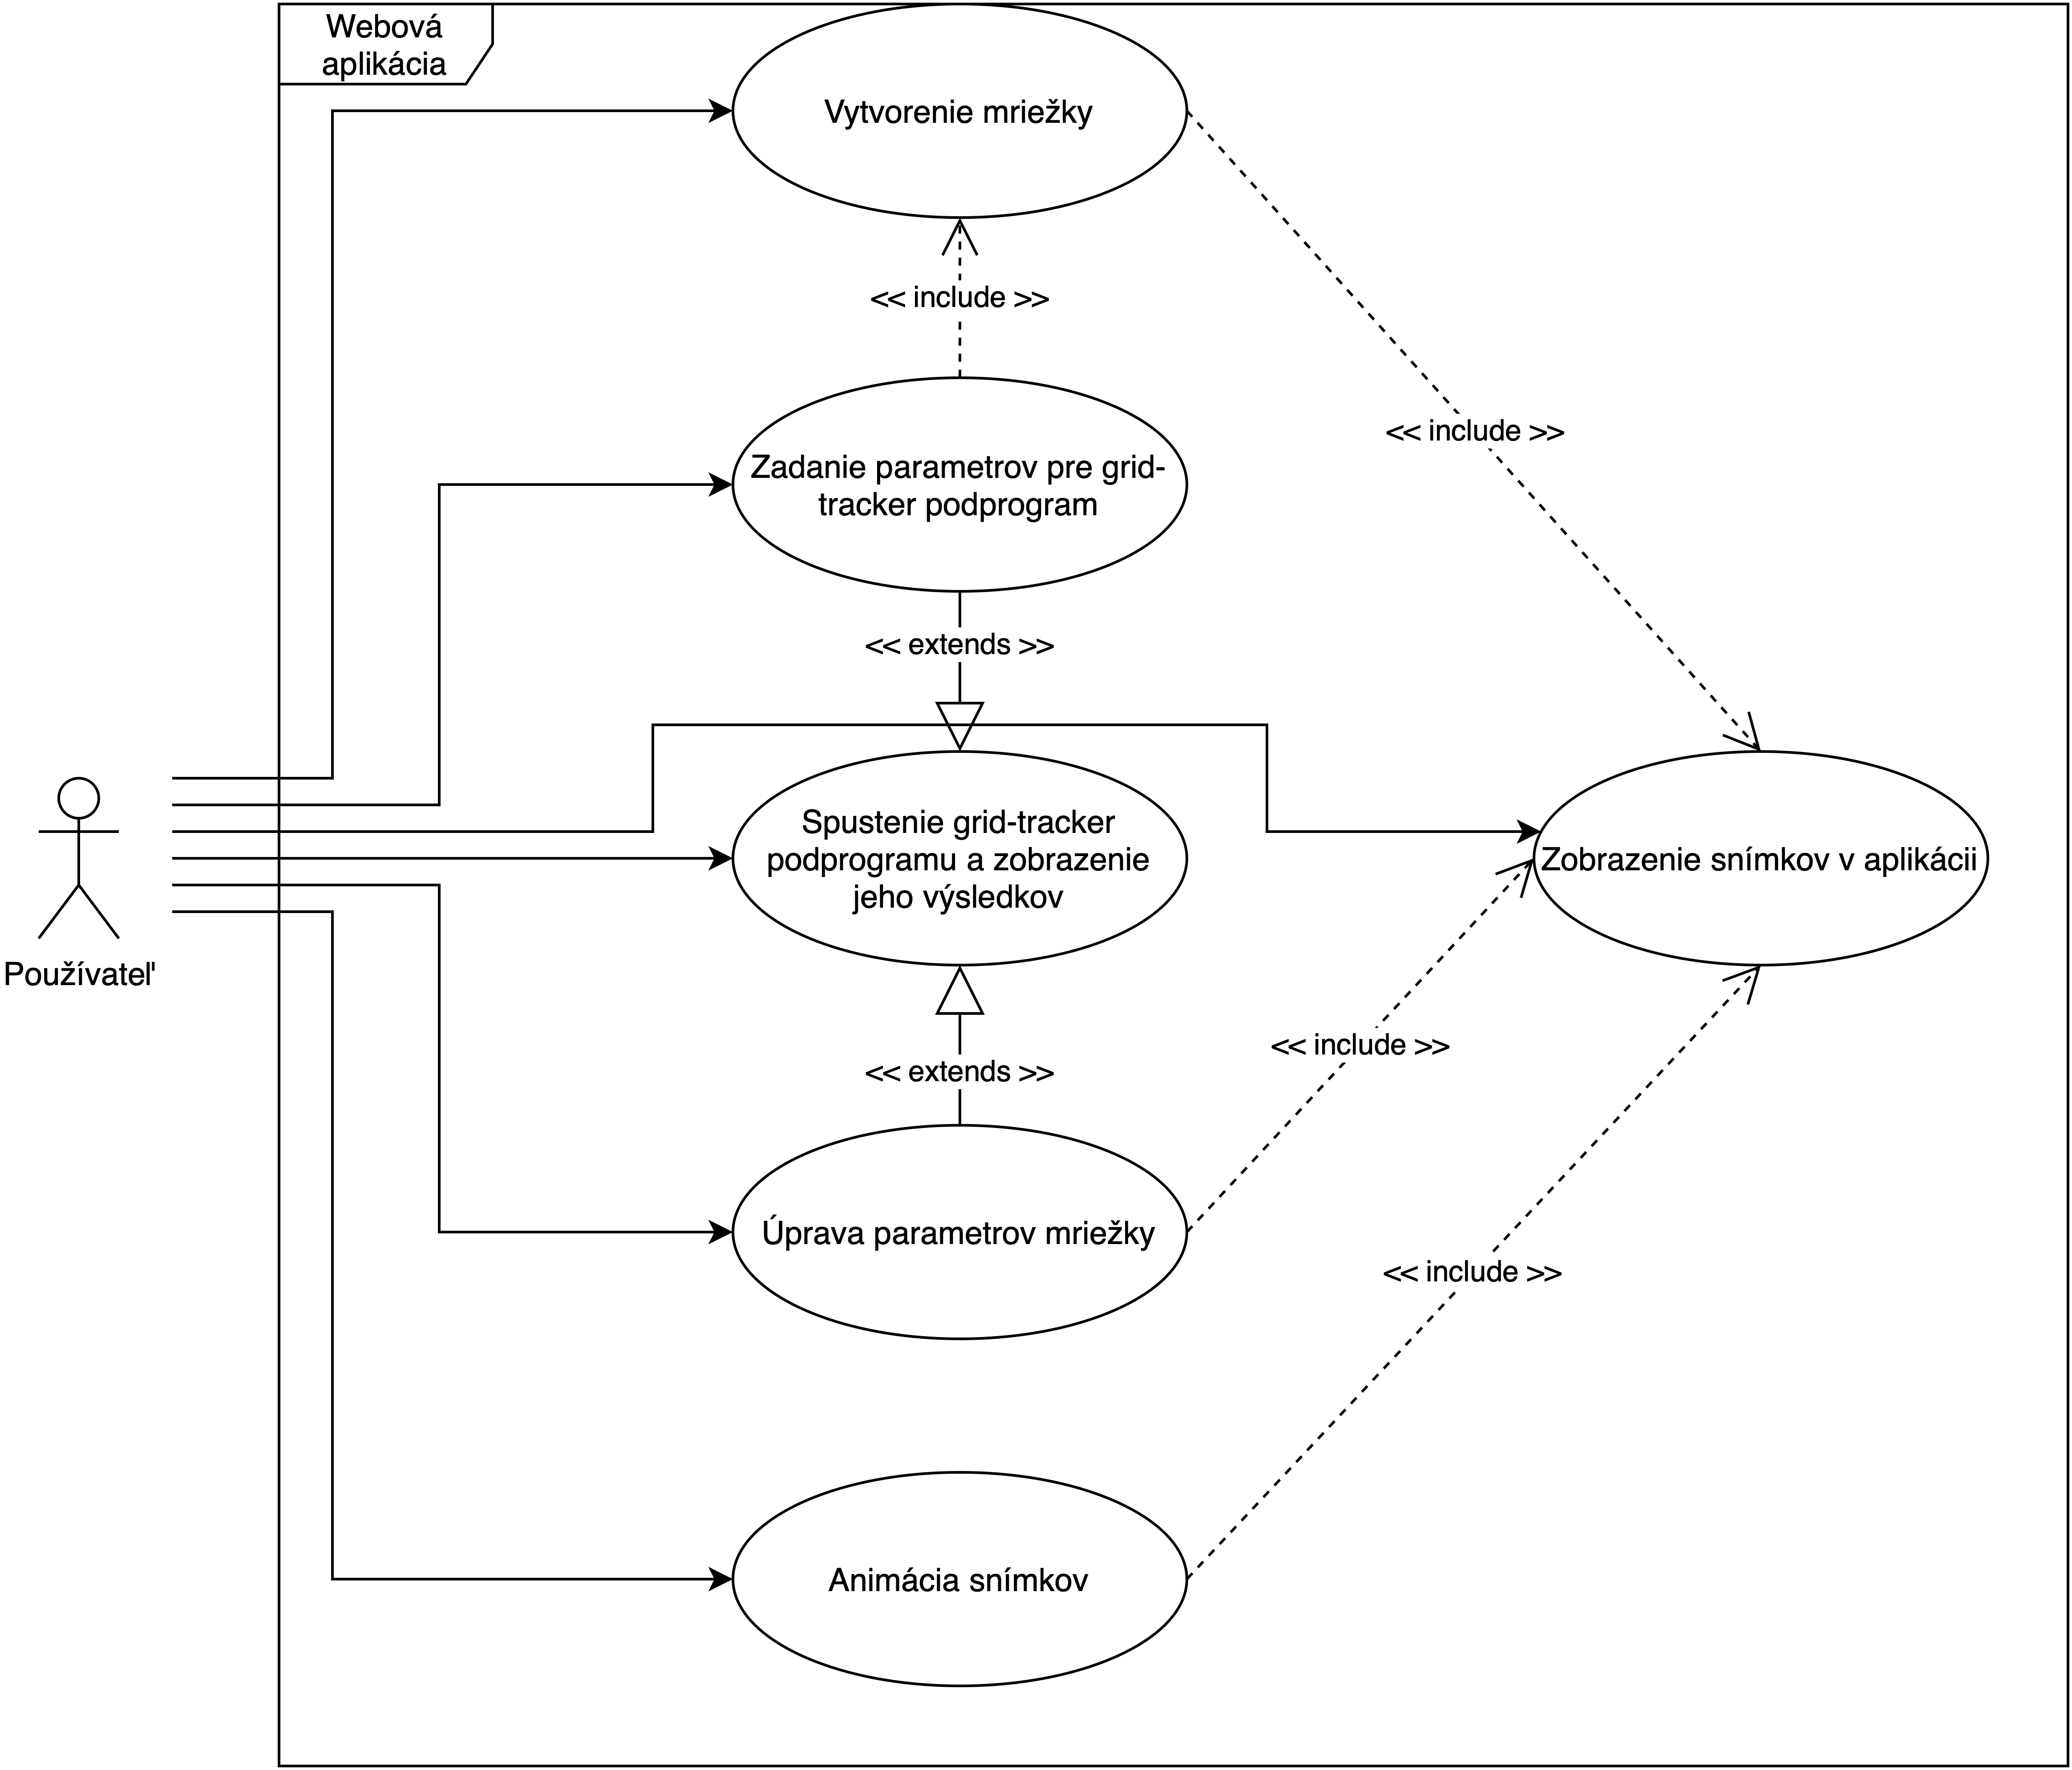
\includegraphics[height=10cm]{media/graphs/usecase.png}
        \captionsetup{justification=centering}
        \captionof{figure}[Use case diagram]{Use case diagram}
\end {center}

\subsection {UC1 -- Zobrazenie snímkov v aplikácii}\label{uc1}
Zobrazenie snímkov magnetickej rezonancie v DICOM formáte je jedným z esenciálnych funkčných požiadaviek -- \uv{\nameref{fr1}}. Nasledovný scenár túto požiadavku realizuje.

\subsubsection*{Scenár:}
\begin {enumerate}
\item {Používateľ klikne na jedno z tlačidiel pre import DICOM snímkov do aplikácie.}
\item {Prehliadač zobrazí systémové okno, v ktorom si používateľ vyberie snímky, ktoré by chcel mať zobrazené v aplikácii.}
\item {Následne potvrdí import želaných snímkov kliknutím na tlačidlo \uv{Otvoriť}.}
\item {Aplikácia automaticky vykreslí prvý importovaný snímok a taktiež zobrazí náhľady ostatných importovaných snímkov.}
\item {V prípade, že sa medzi zvolenými snímkami nachádza súbor, ktorý nekorešponduje so štruktúrou DICOM súboru, aplikácia zobrazí notifikáciu o neúspešnom zobrazení snímky.}
\end {enumerate}
	
\subsection {UC2 -- Animácia snímkov}
Nasledovný scenár realizuje funkciu prehrania série snímkov ako animáciu, ako bolo popísané vo funkčnej požiadavke \uv{\nameref{fr2}}.
Okrem iného taktiež zahŕňa prípad \uv{\nameref{uc1}}. 

\subsubsection*{Scenár:}
\begin {enumerate}
\item {\nameref{uc1}.}
\item {Kliknutím na tlačidlo reprezentujúce štart animácie sa spustí animácia importovaných snímkov.}
\item {Kliknutím na tlačidlo reprezentujúce koniec animácie sa animácia skončí.}
\end {enumerate}

\subsubsection*{Alternatívny scenár:}
\begin {enumerate}
\item [\textbf{2.}] {Používateľ si nastaví rýchlosť animácie, index snímku, od ktorého má animácia začínať alebo index snímku, ktorým má animácia končiť.}
\item  [\textbf{3.}] {Kliknutím na tlačidlo reprezentujúce štart animácie sa spustí animácia importovaných snímkov.}
\item  [\textbf{4.}] {Kliknutím na tlačidlo reprezentujúce koniec animácie sa animácia skončí.}
\end {enumerate}

\subsection {UC3 -- Vytvorenie mriežky}\label{uc3}
Vytvorenie mriežky nad snímkou z MR je potrebné pre účely analýzu pohybu myokardu. Nasledujúci scenár čiastočne realizuje funkčnú požiadavku -- \uv{\nameref{fr3}}. Taktiež zahŕňa prípad použitia \uv{\nameref{uc1}}.

\subsubsection*{Scenár:}
\begin {enumerate}
\item {\nameref{uc1}.}
\item {Používateľ klikne na tlačidlo \uv{Create grid}.}
\item {Aplikácia zobrazí výzvu pre kliknutie na oblasť snímky, kde má byť mriežka vytvorená.}
\item {Používateľ klikne na oblasť snímky, kde chce vytvoriť mriežku.}
\item {Aplikácia vygeneruje mriežku s predvolenými nastaveniami a zobrazí ju.}
\end {enumerate}

\subsection {UC4 -- Úprava parametrov mriežky}\label{uc4}
Medzi prípady použitia patrí aj úprava parametrov mriežky určenej pre analýzu pohybu srdcového svalu. Nakoľko je najprv potrebné mať mriežku  pred jej úpravou vytvorenú, zahŕňa nasledovný scenár aj jej vytvorenie. Ten taktiež čiastočne realizuje funkčnú požiadavku \uv{\nameref{fr3}}.

\subsubsection*{Scenár:}
\begin {enumerate}
\item {\nameref{uc3}.}
\item {Používateľ upraví jeden alebo viacero parametrov uvedených v \ref{old_ui}.}
\item {Aplikácia následne automaticky vykreslí mriežku na základe upravených parametrov.}
\end {enumerate}

\subsection {UC5 -- Zadanie parametrov pre \texttt{grid-tracker} podprogram}\label{uc5}
Pre spustenie algoritmu zodpovedného pre posun mriežky vytvorenej používateľom voči mriežke vygenerovanej SPAMM technikou je potrebné tomuto algoritmu poslať tri parametre definované v \ref{old_ui}. Nasledujúci scenár tento prípad použitia realizuje spolu s funkčnou požiadavkou -- \uv{\nameref{fr4}}.

\subsubsection*{Scenár:}
\begin {enumerate}
\item {\nameref{uc1}.}
\item {Používateľ zadá číselné hodnoty parametrov \uv{Curvature coefficient}, \newline \uv{Force coefficient} a \uv{Stop time}.}
\end {enumerate}

\subsection {UC6 -- Spustenie \texttt{grid-tracker} podprogramu a zobrazenie jeho výsledku}
Spustenie samotného podprogramu a zobrazenie jeho výsledku (súradnice bodov mriežok) vyžaduje nielen mať importované DICOM snímky v aplikácii, ale aj vytvorenú mriežku s upravenými parametrami a zadanými parametrami pre \texttt{grid-tracker} podprogram. To je dôvodom, prečo tento scenár použitia zahŕňa prípady \uv{\nameref{uc1}}, \uv{\nameref{uc3}}, \uv{\nameref{uc4}} a \uv{\nameref{uc5}}. Samotný scenár realizuje funkčnú požiadavku \uv{\nameref{fr5}}.

\subsubsection*{Scenár:}
\begin {enumerate}
\item {\nameref{uc1}}.
\item {\nameref{uc3}}.
\item {\nameref{uc4}}.
\item {\nameref{uc5}}.
\item {Používateľ kliknutím na tlačidlo \uv{Compute} spustí výpočet pomocou \texttt{grid-tracker} podprogramu.}
\item {Po dokončení výpočtu aplikácia zobrazí mriežky upravené horeuvedeným podprogramom.}
\end {enumerate}

\section {Návrh architektúry webovej aplikácie}
Medzi prvými krokmi pred vývojom samotnej webovej aplikácie je nutné zanalyzovať všetky prípustné možností architektúry navrhovanej aplikácie. V tomto prípade návrh architektúry závisí najmä na prepojení webového rozhrania so súčasnou aplikáciou, a preto je potrebné najprv zanalyzovať všetky dostupné možnosti tohto prepojenia. Po porovnaní dostupných možností prepojenia je nutné zvoliť jednu z nich. Následne bude možné pokračovať s analýzou technológií, ktoré budú použité pre vývoj aplikácie.

Čo sa týka samotného prepojenia súčasnej aplikácie, resp. výpočetného podprogramu \texttt{grid-tracker} s novou webovou aplikáciou, existujú dve možnosti, ako môže daná integrácia prebehnúť. Prvou možnosťou je využitie tzv. C\texttt{++} addons\footnote{https://nodejs.org/docs/latest-v18.x/api/addons.html} technológie, druhou možnosťou sa naskytuje využiť relatívne novú technológiu -- WebAssembly\footnote{https://webassembly.org}.

\subsection {C\texttt{++} addons}
C\texttt{++} addons je technológia, ktorá poskytuje rozhranie medzi C/C\texttt{++} knižnicami a JavaScriptom\footnote{https://developer.mozilla.org/en-US/docs/Web/JavaScript}. Táto technológia je implementovaná v rámci Node.js\footnote{https://nodejs.org/en}, čo je behové prostredie JavaScriptu, ktoré bude popísané v samostatnej sekcii.
C\texttt{++} addons umožňuje pristupovať k natívnym API operačného systému a taktiež pomáha integrovať C/C\texttt{++} knižnice tretích strán pre ich priame použitie v Node.js. Doporučeným spôsobom písania takýchto addonov je pomocou technológie Node-API\footnote{https://nodejs.org/docs/latest-v18.x/api/n-api.html}, pomocou ktorej je možné vytvoriť Node-API addon v jazyku C. Pre písanie Node-API addonov v C\texttt{++} je ale potrebné použiť modul \texttt{node-addon-api}\footnote{https://github.com/nodejs/node-addon-api}, nakoľko ten obsahuje hlavičkové súbory v C\texttt{++} \cite{cpp_addons} (vlastný preklad).

Výhodou použitia Node-API technológie je jej nemennosť v rámci rôznych verzií Node.js, čo zaručuje použitie skompilovaného addonu v rôznych verziách Node.js bez nutnosti prekompilovania samotného addonu \cite{cpp_addons} (vlastný preklad).

Nástrojom pre zostavenie takéhoto modulu je build systém \texttt{node-gyp}\footnote{https://github.com/nodejs/node-gyp}. Ten používa \texttt{binding.gyp} súbor, ktorý špecifikuje konfigurácie zostavenia modulu. Táto konfigurácia zahŕňa okrem iného aj cestu k zdrojovým \texttt{.cpp} a \texttt{.h} súborom. Tie musia byť pred samotným zostavením upravené tak, aby používali Node-API rozhranie \cite{cpp_addons} (vlastný preklad).

To zahŕňa vytvorenie metód, ktoré budú prijímať vstupné a výstupné argumenty pretypované na typy pochádzajúce z Node-API.

Pred zostavením addonu je potrebné vygenerovať Makefile pre cieľový operačný systém pomocou príkazu \texttt{node-gyp configure}. Pre samotné zostavenie addonu je následne potrebné exekuovať príkaz \texttt{node-gyp build}. Ten skompiluje želané súbory špecifikované v \texttt{binding.gype} do jediného súboru s príponou \texttt{.node}. Ten je následne možné importovať ako modul do iného JavaScript modulu pomocou kľúčového slova \texttt{import}\footnote{https://developer.mozilla.org/en-US/docs/Web/JavaScript/Reference/Statements/import}. Po importovaní daného modulu je možné volať jeho metódy rovnakým spôsobom ako iné JS metódy \cite{cpp_addons} (vlastný preklad).

\subsection {WebAssembly}
WebAssembly je nový typ jazyku, ktorý je možné exekuovať vo všetkých moderných webových prehliadačoch. Jeho hlavnou výsadou je zvýšenie rýchlosti exekuovania kódu oproti JavaScriptu blížiaci sa k skoro natívnej exekúcii kódu naprogramovaného v jazykoch C, C\texttt{++} alebo Rust\footnote{https://www.rust-lang.org} a iné. Je navrhnutý tak, aby mohol fungovať spoločne s JavaScriptom \cite{webassembly_concepts} (vlastný preklad).

Webová platforma sa dá vo všeobecnosti rozdeliť na dve časti:
\begin{itemize}
\item {VM, pomocou ktorej sa exekuuje kód webovej aplikácie a}
\item {webové API, ktoré je poskytnuté vývojárom pre kontrolu rozličných funkcionalít webového prehliadača, resp. zariadenia  \cite{webassembly_concepts} (vlastný preklad).}
\end{itemize}

Historicky, VM umožňovala načítať len kód napísaný v JavaScripte. Avšak postupom času sa ukázalo, že JS nie je určený pre aplikácie, ktoré potrebujú dosahovať väčší výpočetný výkon, ako sú napr. 3D hry, VR/AR, editácia videa či obrázkov a iné.
WebAssembly bolo navrhnutý tak, aby tieto problémy vyriešil a priniesol prostriedky pre vývoj takýchto aplikácií. 
Pomocou WebAssembly JS API\footnote{https://developer.mozilla.org/en-US/docs/WebAssembly/Using\textunderscore the\textunderscore JavaScript\textunderscore API} je možné načítať WebAssembly moduly -- čo sú moduly v binárnom formáte -- do JavaScript aplikácie a zdieľať s touto aplikáciou funkcionalitu poskytovanú týmito modulmi \cite{webassembly_concepts} (vlastný preklad).

Možností, ako daný modul vytvoriť, je viacero:
\begin {itemize}
\item {portovať C/C\texttt{++} aplikáciu pomocou technológie Emscripten\footnote{https://emscripten.org},}
\item {písať priamo vo WebAssembly,}
\item {napísať aplikáciu v inom jazyku a kompilovať ju pomocou kompilátora podporujúci WebAssembly výstup, alebo}
\item {použiť AssemblyScript\footnote{https://www.assemblyscript.org}, ktorý je podobný TypeScript\footnote{https://www.typescriptlang.org} jazyku a dá sa priamo skompilovať do WebAssembly  \cite{webassembly_concepts} (vlastný preklad).}
\end {itemize}

Nakoľko sa v tomto prípade jedná o C\texttt{++} aplikáciu -- konkrétne \texttt{grid-tracker} podprogram -- bude bližšie analyzovaná prvá možnosť z dostupných možností.

V rámci nej je potrebné stiahnuť a nainštalovať si Emscripten kompilátor. Ten umožňuje skompilovať program v C/C\texttt{++} do modulu vo formáte \texttt{.wasm} \cite{cpp_to_wasm} (vlastný preklad).

Následne je možné daný C\texttt{++} program skompilovať pomocou príkazu \texttt{em++ sample.cpp -o sample.html}. Výstupom tohto príkazu sú tri súbory -- \newline \texttt{a.out.js}, \texttt{a.out.wasm} a \texttt{sample.html}. Prvý zo súborov tvorí JS kód, ktorého úloha je prepojiť daný WASM modul (druhý súbor) s JS prostredím. Následne je možné tento modul spolu s JS kódom importovať do HTML\footnote{https://developer.mozilla.org/en-US/docs/Web/HTML} stránky, na ktorej daný modul pobeží. Takto importovaný kód v HTML stránke je možné vidieť v súbore \texttt{sample.html} \cite{cpp_to_wasm} (vlastný preklad).

Celý proces je pre ilustráciu zobrazený na obrázku nižšie:
\begin {center}
        \centering
        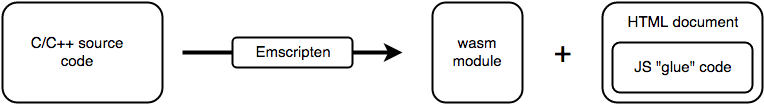
\includegraphics[height=1.75cm]{media/graphs/cpp_to_wasm.png}
        \captionsetup{justification=centering}
        \captionof{figure}{Od zdrojového kódu k .wasm modulu \cite{cpp_to_wasm_image}}
\end {center}

\subsection {Výsledná voľba prepojenia}
C\texttt{++} addons technológia je, ako bolo uvedené, implementovaná v Node.js, čo by v prípade zvolenia tejto technológie znamenalo zvolenie architektúry klient-server. Klientom by bol v tomto prípade webový prehliadač, ktorý by posielal HTTP požiadavku serveru s potrebnými dátami pre \texttt{grid-tracker} podprogram. Po výpočte by server v odpovedi na danú požiadavku poslal klientovi informácie o bodoch a úsečkách, ktoré by mali byť vykreslené na všetkých importovaných snímkoch magnetickej rezonancie.

V prípade použitia technológie WebAssembly by všetky výpočetné operácie mohli byť implementované na úrovni klienta. Tým pádom by nebolo nutné posielať žiadne dáta serveru, čo hrá v prospech bezpečnosti. Avšak, ako z analýzy \texttt{grid-tracker} podprogramu vyplýva, \texttt{grid-tracker} a knižnica TNL pre zrýchlenie výpočetných algoritmov používajú OpenMP technológiu.
Bohužiaľ, WebAssembly túto technológiu nepodporuje, čo by v tomto prípade znamenalo, že by celý výpočet musel prebiehať jednovláknovo alebo byť refaktorovaný, aby používal viacero vlákien pomocou technológie WebAssembly threads \cite{webassembly_threads}.

Čo sa týka použitia C\texttt{++} addons, ten OpenMP technológiu podporuje. Taktiež by bol v rámci tejto technológie nutný menší zásah do samotného zdrojového kódu \texttt{grid-tracker} podprogramu, nakoľko by stačilo vytvoriť jednu wrapper funkciu v C\texttt{++}, ktorá by bola zodpovedná za konverziu dát do potrebného formátu a taktiež za vrátenie výsledku. Doterajší kód by mohol zostať prakticky nezmenený, resp. s minimálnymi zmenami.
Taktiež nie je možné spoľahnúť sa na to, že by webové prehliadače, na ktorých by bežala nová webová aplikácia, podporovala WebAssembly technológiu. Rovnakým spôsobom je možné argumentovať ohľadom výkonu zariadení, na ktorých by daný výpočetný algoritmus bežal, v prípade WebAssembly.

Na základe týchto dôvodov je praktickejšie vybrať si technológiu C\texttt{++}, s ktorou by mala byť implementácia prepojenia \texttt{grid-tracker} podprogramu a webovej aplikácie nie len rýchlejšia, ale s podporou OpenMP technológie. Výpočty v rámci \texttt{grid-tracker} podprogramu by taktiež neboli závislé na dostupných výpočetných prostriedkov klienta, ale serveru, čo umožňuje mať väčšiu kontrolu nad potrebným škálovaním výkonu pre \texttt{grid-tracker} podprogram. 

\section {Technológie pre vývoj webovej aplikácie}
Po analýze, ako bude webová aplikácia prepojená s \texttt{grid-tracker} podprogramom, je nutné zvoliť potrebné technológie, ktoré budú použité pri vývoji webovej aplikácie. V rámci tejto sekcii nebudú popísané žiadne konkrétne balíčky a iné závislosti.

\subsection {HTML5}
Pre definovanie štruktúry webového dokumentu a jeho významu bude potrebné použiť značkovací jazyk HTML. Tento jazyk pozostáva zo série značiek (elementov) a k nim príslušných atribútov, pomocou ktorých je možné vytvorený obsah anotovať a významovo ho definovať. Týmto spôsobom je možné vytvoriť nadpisy, odstavce textu, číselné i nečíselné zoznamy, či importovať obrázky alebo sprostredkovať audio/video, atď. Takto štruktúrovaný obsah definovaný pomocou jazyka HTML je možné zobraziť v ľubovoľnom webovom prehliadači podporujúcom tento jazyk. Webový prehliadač takýto dokument zanalyzuje a na základe použitých značiek vykreslí. Každá značka má definovaný predvolený štýl zobrazenia, ktorý sa môže líšiť od prehliadača k prehliadaču.

Nižšie je uvedený príklad základnej štruktúry HTML5 webového dokumentu:
\begin{lstlisting}[language=HTML]
<!doctype html5>
<html>
  <head></head>
  <body>
    <p>Hello world!</p>
  </body>
</html>
\end{lstlisting}

Značka \texttt{<!doctype>} definuje verziu použitého HTML dokumentu, čo je v tomto prípade HTML5. Ďalej nasleduje značka \texttt{<html>}, ktorej úloha je zoskupiť elementy \texttt{<head>} a \texttt{<body>}. V elemente \texttt{<head>} sa zvyčajne nachádzajú metadáta ako názov dokumentu, špecifikácia ďalších zdrojov pre načítanie v dokumente a iné. Na druhú stranu, element \texttt{<body>} zoskupuje obsah dokumentu, ktorý je zobrazený prehliadačom.

Prvá verzia tohto jazyka -- HTML 2.0\footnote{https://www.ietf.org/rfc/rfc1866.txt} -- bola definovaná v roku 1995 samotným vynálezcom WWW, Timom Berners-Leeom. Momentálne najnovšou verziou HTML jazyka je tzv. HTML5 Living Standard\footnote{https://html.spec.whatwg.org}, ktorá priniesla viacero nových značiek definovanými v HTML štandarde, ako napr. značku \texttt{<audio>} pre prehrávanie audia, \texttt{<video>} pre prehrávanie videa, či \texttt{<picture>}, ktorá je určená pre definovanie viacero zdrojov pre zobrazený obrázok. Okrem samotných značiek, HTML5 štandard taktiež poskytuje niekoľko API, ktoré sú implementované v samotných webových prehliadačoch. Pomocou týchto API je možné napr. geolokalizovať používateľa pomocou HTML5 Geolocation API alebo vykreslovať grafiku použitím HTML5 Canvas API, a iné.

\subsection {CSS 3}
CSS\footnote{https://developer.mozilla.org/en-US/docs/Web/CSS} -- z anglického Cascading Style Sheets -- je jazyk popisujúci vzhľad použitých HTML5 elementov vo webovom dokumente. Tento jazyk definuje súbor pravidiel, ktoré môžu byť aplikované na jednotlivé elementy webového dokumentu, na základe ktorých sa mení vzhľad pravidlami ovplyvnených elementov.

Samotné pravidlo sa skladá zo selektora, ktorý definuje rozsah elementov, ktoré budú ovplyvnené. Nasleduje zoznam vlastností s ich hodnotami, ktoré majú byť aplikované na samotný selektor. Týmto spôsobom je možné definovať vzhľad nie len jedného, ale aj viacerých elementov vo webovom dokumente pomocou jedného pravidla.

Nižšie je uvedený príklad pravidla, ktoré mení farbu textu vo všetkých elementoch \texttt{p} (\texttt{p} definuje odstavec textu) na červenú:

\begin{lstlisting}
p {
    color: red;
}
\end{lstlisting}

Zoskupené pravidlá sa väčšinou ukladajú do samostatného súboru s príponou \texttt{.css}. Tento súbor je následne nalinkovaný do HTML5 dokumentu pomocou značky \texttt{link}, ktorú prehliadač pri parsovaní dokumentu prečíta a následne aplikuje.

Definovanie samotného selektoru môže byť pre dané pravidlo sofistikovanejšie než ako bolo ukázané v príklade vyššie. Element môže byť špecifikovaný na základe jeho rôznych atribútov, ako ID, zoznam tried, či hodnotou jeho atribútu, atď.

Čo sa týka verzíí CSS jazyka, u CSS sa nepoužívajú verzie ale tzv. levely. Prvým levelom bol CSS Level 1, ktorý sa stal odporúčanou špecifikáciou W3C konzorcia\footnote{https://www.w3.org} o rok neskôr ako HTML 2.0, v 1996. Tento level bol základom pre nasledujúce levely tohto jazyka. V súčasnosti najnovší level CSS jazyka je CSS Level 3, v ktorom sa narozdiel od predchádzajúcich levelov jednotlivé časti jazyka delia na moduly, z ktorých každý môže mať level vyšší než samotná špecifikácia. Z tohto dôvodu sa taktiež rozhodlo, že samotný level CSS jazyka sa už nebude zvyšovať.

\subsection {JavaScript}
JavaScript je cross-platformový skriptovací programovací jazyk a treťou základnou technológiou pre vývoj webových stránok a aplikácií, spolu s HTML a CSS. Používa sa pre implementovanie funkcionality, kde kombinácia HTML a CSS nie je pre daný účel vhodná alebo určená, ako napr. dynamická interakcia používateľa s webovou stránkou/aplikáciou, riešenie rôznych výpočetných úloh, odosielanie dát na server a prijímanie odpovede, a iné.

Samotný jazyk bol vytvorený Brendanom Eichom, pracujúcom vo firme Netscape, ktorá taktiež vyvíjala webový prehliadač -- Netscape Navigator. JavaScript bol zahrnutý už vo verzii 2.0 tohto prehliadača, ktorý bol vydaný v roku 1995. Následne sa začal objavovať aj v iných prehliadačoch -- napr. vo všetkých prehliadačoch vytvorených firmou Microsoft počnúc Internet Explorerom 3.0. 

JavaScript nasleduje ECMAScript špecifikáciu\footnote{https://tc39.es/ecma262/}, vytvorenú Ecma International organizáciou. Tá kontinuálne vydáva každý rok novú štandardizovanú ECMAScript špecifikáciu, ktorá slúži ako predloha pre vytvorenie všeobecného skriptovacieho jazyka. JavaScript je v tomto prípade jazyk spĺňajúci tento štandard, nakoľko sa ním riadi a implementuje ho. Momentálne najnovšou verziou štandardu je jeho 14. edícia, ktorá pridala najmä nové metódy pracujúce s poľom (\texttt{Array}).

Čo sa týka vlastností samotného jazyka, JavaScript je dynamicky typovaným jazykom, čo znamená, že pri vytváraní premenných sa nedefinuje ich typ. To umožňuje do rovnakej premennej na jednom mieste uložiť číslo, a na inom zase reťazec. Taktiež sa jedná objektovo-orientovaný jazyk, kde dedičnosť je riešená mechanizmom prototypov, kde metódy a vlastnosti môžu byť za behu pridané do akéhokoľvek objektu. Taktiež používa primárne jedno hlavné vlákno pre všetky svoje operácie, avšak je možné vytvoriť tzv. pracovné vlána pomocou Web Workers technológie. Nakoľko JavaScript podporuje OOP, imperatívny a deklaratívny štýl písania kódu, jedná sa o tzv. multi-paradigmatový jazyk.

\subsubsection {Typescript}

\subsection {Node.js}

\subsection {Docker}

\section {Analýza spracovania MR snímkov vo webovej aplikácii}
Spracovávanie importovaných MR snímkov by v aplikácii malo prebiehať najmä na strane klienta -- vo webovom prehliadači. Takto zvolený prístup zamedzí prípadnému útočníkovi preniknúť k snímkom a dátam o pacientoch, ktoré by v opačnom prípade museli byť uchovávané na strane servera. Z uvedeného vyplýva, že pre implementáciu aplikácie bude potrebné nájsť JavaScript knižnicu resp. knižnice, ktoré sú schopné spracovať DICOM súbory v prehliadači.

Pod pojmom \uv{spracovať} je myslené: čítanie hlavičky DICOM súborov, zobrazenie snímkov nachádzajúcich sa v týchto súboroch, či tieto snímky modifikovať. Medzi ďalšie požiadavky kladené na takúto knižnicu patrí jej aktívny vývoj, dostupná dokumentácia a taktiež použiteľnosť knižnice pre produkčné nasadenie. Je možné, že neexistuje daná knižnica spĺňajúca všetky požiadavky, ktoré sú na ňu kladené. V takom prípade by mal byť nájdený mix knižníc, ktoré spolu tieto podmienky spĺňajú.

Bohužiaľ, všetky požiadavky kladené na hľadanú knižnicu nespĺňa ani jedna nájdená knižnica, ale výber viacero knižníc, kde každá z nich implementuje určitú časť požiadaviek a dokopy podmienky kladené na knižnicu vyššie, spĺňajú.

Jedná sa o nasledovné knižnice:
\begin {itemize}
\item {Cornerstone Core,}
\item {Cornerstone WADO Image Loader a}
\item {Dicom Parser.}
\end {itemize}

\subsection {Cornerstone Core}
Cornerstone Core\footnote{https://github.com/cornerstonejs/cornerstone} je knižnica, ktorá má za úlohu zjednodušiť proces vývoja komplexnejších webových aplikácií, ktoré majú za úlohu zobrazovať snímky akéhokoľvek formátu, vrátane bežných medicínskych snímkových formátov. Taktiež poskytuje API, pomocou ktorého je možné zobrazovať DICOM snímky a meniť ich vlastnosti, ako napr. zvýšiť alebo znížiť jas, priblížiť snímku alebo ju oddialiť, a iné.
Táto knižnica neimplementuje samotné importovanie DICOM súborov a ich spracovanie. Túto funkcionalitu deleguje na tzv. ImageLoaders. Tie po spracovaní DICOM súborov posunú DICOM dáta cez spoločné rozhranie Cornerstone Core knižnici, ktorá ich nakoniec vykreslí. Cieľom tohto prístupu Cornerstone Core knižnice je jej dôraz na minimalizmus a poskytnutie flexibility pri spracovávaní rôznych typov obrazových dát.

V súčasnosti sa pripravuje nová \uv{Cornerstone Core} knižnica, ktorej názov sa zmení na \uv{Cornerstone3D}\footnote{https://github.com/cornerstonejs/cornerstone3D-beta}. Keďže je táto knižnica momentálne v beta berzii a stabilná verzia tejto knižnice ešte nebola vydaná, vývoj aplikácie bude postavený na doterajšej Cornerstone Core knižnici.
Momentálne neexistuje alternatíva tejto knižnice, ktorá by sa špecifikovala na túto oblasť. 

\subsection {Cornerstone WADO Image Loader}
Cornerstone WADO Image Loader\footnote{https://github.com/cornerstonejs/cornerstoneWADOImageLoader} je tzv. ImageLoader, ktorý je zodpovedný za načítanie a spracovanie DICOM súborov. Použitie tejto knižnice je vynútené samotnou Cornerstone Core knižnicou. Táto knižnica podporuje nie len načítanie DICOM súborov cez HTTP protokol, ale aj z lokálneho súborového systému pomocou File API\footnote{https://developer.mozilla.org/en-US/docs/Web/API/File\textunderscore API} implementovaného webovými prehliadačmi. Po načítaní DICOM súborov je ich parsovanie prenechané knižnici Dicom Parser. Nakoľko sa veľkosť týchto súborov môže pohybovať v rádoch megabajtov (MB), samotné parsovanie súborov beží tiež pomocou webovej technológie zvanej Web Workers\footnote{https://developer.mozilla.org/en-US/docs/Web/API/Web\textunderscore Workers\textunderscore API}. Pre začiatok priblížim technológiu Web Workers a následne knižnicu Dicom Parser\footnote{https://github.com/cornerstonejs/dicomParser}.

\subsubsection {Web Workers}
JavaScript je v prehliadači implementovaný ako jednovláknový jazyk využívajúci jedno hlavné vlákno a exekúcia skriptov tohto jazyka prebieha zvyčajne v tomto vlákne. Výpočetne náročné úlohy by avšak mohli vyústiť do zablokovania tohto vlákna, ktoré sa prejavuje nereagovaním prehliadača na rozličné používateľské akcie alebo nevykreslovaním aktualizácií na webovej stránke. Dôvodom zablokovania hlavného vlákna by v tomto prípade bolo využitie všetkých dostupných prostriedkov prioritne pre danú výpočetne náročnú úlohu. \newline
Web Workers technológia je štandardom, ktorý je implementovaný a poskytovaný webovými prehliadačmi umožňujúci exekúciu takýchto úloh, ktoré by inak pri dlhšom spracovávaní mohli dané hlavné vlákno zablokovať. Pomocou Web Workers je možné predísť zablokovaniu hlavného vlákna jednoduchým vytvorením nového pracovného vlákna pomocou konštruktu \texttt{new Worker(url)}, kde \texttt{url} je adresa skriptu, ktorý má bežať v novom pracovnom vlákne. Takéto pracovné vlákno môže exekuovať JS skript bez zablokovania hlavného vlákna, keďže je od neho nezávislé \cite{using_web_workers}.

\subsection {Dicom Parser}
Dicom Parser je knižnica implementujúca parsovanie všetkých známych validných DICOM súborov. Knižnica je navrhnutá pre beh vo všetkých moderných HTML5 prehliadačoch a k svojej funkčnosti nezávisí na iných knižniciach. Dicom Parser poskytuje globálny objekt \texttt{dicomParser}, ktorý obsahuje viacero metód, z ktorých je najzaujímavejšia metóda \texttt{parseDicom}. Argumentom tejto metódy je \texttt{Uint8Array} pole obsahujúce nespracovaný (raw) obsah DICOM súboru. Výsledkom volania tejto metódy spolu s \texttt{Uint8Array} poľom je \texttt{DataSet} objekt obsahujúci vyparsovaný obsah DICOM súboru.

Alternatívou Dicom Parser knižnice by mohla byť knižnica \texttt{dcm.js}\footnote{https://github.com/dcmjs-org/dcmjs}, avšak vývoj tejto knižnice nie je stále dokončený (nebola zatiaľ vydaná jej stabilná verzia) a sami vývojári varujú pred použitím tejto knižnice v produkčnom prostredí. \todo {pridaj citáciu}

Pre zhrnutie informácií v tejto sekcii -- knižnica Cornerstone WADO Image Loader využíva Web Workers pre vytvorenie nových pracovných vlákien, ktorých úloha je parsovanie DICOM súborov pomocou metódy \texttt{parseDicom} objektu \texttt{dicomParser} pochádzajúceho z Dicom Parser knižnice uvedenej vyššie. Metódou vrátený \texttt{DataSet} objekt je následne poslaný knižnici Cornerstone Core, ktorá sa postará o vykreslenie vyparsovaného DICOM snímku z tohto objektu.

Nasledujúca sekcia sa bude zaoberať analýzou a návrhom, ako vykresliť mriežku na zobrazenú DICOM snímku pomocou knižnice Cornerstone Tools.

\section {Analýza vykreslenia mriežky nad MR snímkami}
Keďže bude nie len potrebné MR snímky zobrazovať, ale aj nad týmito snímkami vykreslovať používateľom generovanú mriežku (ako bolo uvedené vo funkčnej požiadavke \ref{fr3}), je nutné nájsť knižnicu, ktorá vykresľovanie takejto mriežky nad určitou oblasťou MR snímky podporuje.

\subsection {Cornerstone Tools}
Tou knižnicou je Cornerstone Tools\footnote{https://github.com/cornerstonejs/cornerstoneTools} knižnica, ktorá asistuje nie len pri vytváraní rôznych anotácií pre DICOM snímky načítané pomocou Cornerstone Core, ale aj pri ich segmentácii či rôznych meraní. Táto knižnica ponúka široký počet nástrojov, ktoré môžu dané snímky modifikovať alebo nad týmito snímkami vykreslovať rôzne informácie či lomené čiary.
Prednosťou tejto knižnice je API, pomocou ktorého je možné vytvárať nové nástroje, manažovať ich, či importovať/exportovať ich stav. Pre využitie tejto knižnice je potrebná nie len Cornerstone Core knižnica, nakoľko je s ňou úzko previazaná, ale aj knižnica \texttt{Hammer.js}\footnote{https://github.com/hammerjs/hammer.js} a Cornerstone Math\footnote{https://github.com/cornerstonejs/cornerstoneMath}.

Cornerstone Tools využíva Cornerstone Core knižnicu pre reagovanie na rôzne eventy, ktoré Conerstone Core knižnica emituje. Na základe týchto eventov môžu nástroje Cornerstone Tools knižnice meniť svoj stav.
\texttt{Hammer.js} knižnica implementuje podporu rozhrania založeného na dotyku namiesto myši. Túto knižnicu je potrebné importovať bez ohľadu na to, či sa plánujú využívať gestá na báze dotyku alebo nie, nakoľko niektoré nástroje sú od tejto knižnice závislé.
Cornerstone Math, ako už názov napovedá, poskytuje rôzne matematické operácie prevažne týkajúce sa vektorovej matematiky. Niektoré nástroje z Cornerstone Tools knižnice ju používajú napr. pre výpočet vzdialenosti medzi rôznymi bodmi.

Nakoľko Cornerstone Tools neobsahuje mriežku ako nástroj, ktorý vie knižnica zobraziť a s ňou ďalej pracovať, bude nutné túto mriežku od základov implementovať. Implementácia tejto mriežky môže využívať API poskytované samotnou knižnicou, pomocou ktorej by bolo možné danú mriežku implementovať bez zásahu do samotnej knižnice alebo bude nutné danú mriežku naprogramovať priamo do tejto knižnice.

Obe možnosti implementácie majú svoje výhody a nevýhody.
Pri implementácii mriežky pomocou dedikovaného API by nebolo potrebné udržiavať vlastnú kópiu Cornerstone Tools knižnice. V tomto prípade by pre využitie rôznych funkcií implementovaných v samotnej knižnici bolo možné vyžadovanú funkcionalitu importovať pomocou metódy \texttt{importInternal(moduleName)}. Nevýhodou tohto spôsobu je nedostatočná flexibilita spojená s nemožnosťou importovania všetkej funkcionality, ktorá by mohla byť pri vývoji potrebná. Ďalším negatívom zvolenia tohto spôsobu by bola nemožnosť upravenia akéhokoľvek kódu v Cornerstone Tools knižnici.
Na druhú stranu, ak by mala byť mriežka implementovaná priamo v Cornerstone Tools knižnici, odpadol by problém s importovaním teoreticky potrebnej funkcionality, nakoľko by sa dal importovať akýkoľvek modul knižnice priamo pomocou JS konštruktu \texttt{import}, bez nutnosti využitia \texttt{importInternal} metódy.
Nakoľko v tomto momente nie je jasné, či bude výsledná implementácia mriežky potrebovať zmenu niektorého zo súborov Cornerstone Tools knižnice, je vhodnejšie začať implementovať mriežku priamo v knižnici. Keď bude implementácia tejto mriežky dokončená, bude nutné posúdiť, či je možné celú funkcionalitu mriežky migrovať do riešenia využívajúceho iba dedikované API pre svoju funkcionalitu.  \todo {v implementácii zhodnotiť že to nie je možné, nakoľko boli potrebné zmeny v samotných súboroch cornerstone tools}.

Ako pri Cornerstone Core, tak aj Cornerstone Tools knižnica bude mať čoskoro svojho nástupcu, knižnicu Cornerstone Tools v2\footnote{https://github.com/cornerstonejs/cornerstone3D-beta/tree/main/packages/tools}, ktorá bude určená pre Cornerstone3D. Táto nová knižnica je momentálne v aktívnom vývoji a jej stabilná verzia ako v prípade Cornerstone3D nebola stále vydaná. To je dôvodom, prečo bude pri implementácii aplikácie použitá doterajšia verzia Cornerstone Tools knižnice.

\section {Analýza frameworkov pre tvorbu webovej aplikácie}
%Webovú aplikáciu je možné od základov naprogramovať len pomocou vlastného kódu, avšak takýto vývoj by bol zdĺhavejší a vývojár by sa musel sústrediť na veci, ktoré by nemuseli byť pri vývoji relevantné. Preto existujú frameworky, ktoré vývojára od takejto práce odbremenia.Pre vývoj webovej aplikácie bude potrebný fullstack framework, ktorý sa zameriava nie len na frontendovú časť, ale aj na backendovú časť aplikácie. Nakoľko  Výhodou fullstack frameworku oproti použitiu frameworkov zvlášť pre frontend a pre backend je potreba ovládania len jedného frameworku, spoločný základ pre frontend a backend a tým pádom jednoduchšie zostavenie aplikácie.

%V súčasnosti sú najviac používané fullstackové frameworky pre webové aplikácie nasledujúce:
%Next.js
%Nuxt.js

\subsection {Next.js}

\subsection {Nuxt.js}

\subsection {Výsledná voľba frameworku}

\section {Návrh používateľského rozhrania}

\todo {pridať wireframe}

\section {Návrh prepojenia webového rozhrania so súčasnou aplikáciou}

\subsection {Anonymizácia DICOM dát}

\subsection {Komunikácia medzi serverom a klientom}
\todo {pridať diagram komunikácie}

